\chapter{\label{cha:c11tester}Fuzzing with C11Tester}

C11Tester is an automatic testing tool that supports a large fragment of C/C++ weak memory model. This chapter presents an overview of C11Tester and customization points of its pluggable framework. It then describes the fuzzer's implementation. Finally, we show the evaluation results on several benchmarks.

\section{Overview of C11Tester}

C11Tester contains the following basic constructs: instrumentation, scheduler, consistency checker and race detector.

C11Tester uses an LLVM pass, CDSPass, to instrument all atomic operations, non-atomic accesses to shared memory locations, thread functions, mutex operations, and fence operations by inserting corresponding function calls. The compiled program is linked with a dynamic library containing these function calls.
C11Tester implements a thread library that supports the same APIs of C++'s standard library and POSIX thread library. The user's thread function calls will be mapped into user space fibers, instead of kernel space threads. Thus, all threads are executed sequentially, with scheduling managed by a central scheduler provided by C11Tester. A context-switching approach is used to simulate thread interleavings and improve efficiency.
Each atomic operation, thread creation and joining, mutex locks and unlocks, and memory fences will create an Action object, containing its type, value, memory order, thread ID and other runtime information. Since all threads are sequenced during execution, each action has a unique sequence number. The relations between actions, such as read from and synchronized with, are also maintained by the Action class.

Although C/C++ programs under weak memory models do not use scheduling semantics, C11Tester does contain a central scheduler. It is worth noting that the scheduler does not simulate schedulings of threads, instead, it is designed to check actions of different threads in a total order. This is based on the implementation of mapping user's threads into fibers and checking them sequentially. All actions within the same thread will be checked following their sequence order, as a step, and the scheduler decides whether to check actions of other threads in the next step. Hence, two decisions will be made at each step, the behavior of the current action and the next thread to select. If the current action is a read, C11Tester will choose a write action for it to read from. Since the read-modify-write operations are instrumented with two functions, a read and a write, the scheduler ensures these two actions are atomic, i.e.  they are checked without switching to other threads in between.

Memory locations are divided into two types: atomic locations and non-atomic locations. Non-atomic access to shared memory locations is the source of data races. C11Tester implements a race detector to check data races. The race detector allocates a chunk of shadow memory for each of the non-atomic memory locations. Loading from or writing to non-atomic shared variables is instrumented with specific functions, which will register the current thread's state to the shadow memory. When multiple concurrent accesses to some shared non-atomic memory with at least one of them being a write is detected, a data race will be reported.

Here, we use an example to demonstrate the process of C11Tester's random testing procedure.

\begin{lstlisting}[caption={P3}, label={P3}]
#include "librace.h"
#include <atomic>
#include <thread>
uint8_t data = {};
std::atomic<int> flag = { 1 };  

// thread 2
void t2() {
    store_8(&data, 0);          // cds_store8    
    flag.store(1, mo_release); 
}

// thread 3
void t3() {
    if (flag.load(mo_acquire))
        store_8(&data, 1);
}

// thread 1
int main() {
    std::thread thrd2(t2);
    std::thread thrd3(t3);
    thrd2.join();
    thrd3.join();
}
\end{lstlisting}

In this program, there are two shared variables: a non-atomic variable \texttt{data} and an atomic flag. The \texttt{librace.h} header is provided by C11Tester and contains the instrumented function \texttt{store\_8} for non-atomic variables. The initialization of \texttt{flag}, which is non-atomic, deliberately uses 1 as the initial value. Since the C++ standard thread library internally calls POSIX APIs, the thread-related function calls will be hooked by C11Tester's dynamic library.

After compilation, the random tester launches the program. After initializing the global variables, the checker creates the first thread, which is the \texttt{main} thread, and assigns an tid, 1, to it. The first event is the creation of \texttt{thrd2}. After \texttt{thrd2} is created and assigned an tid of 2, two threads, \texttt{main} and \texttt{thrd2}, are active. The tester will randomly pick a thread to continue. Suppose the \texttt{main} thread is selected; the next event of it is the creation of \texttt{thrd3}. After creating \texttt{thrd3}, the next event of main is joining \texttt{thrd2}, making \texttt{main} inactive. Now, the current active threads are: \texttt{thrd2} and \texttt{thrd3}.

If the tester selects \texttt{thrd2}, the two events in it, writing to \texttt{data} and \texttt{flag}, will be consumed, and the \texttt{thrd2} is finished. Now, \texttt{thrd2} becomes joinable and the currently active threads are: \texttt{main} and \texttt{thrd3}. Suppose \texttt{main} is selected and after joining \texttt{thrd2} it becomes inactive again. Then, \texttt{thrd3} becomes the only active thread so it will be executed without the need to make a choice. The first event in \texttt{thrd3} is loading the value of \texttt{flag}. Since the store of \texttt{flag} in \texttt{thrd2} has already been explored, the non-atomic initialization of \texttt{flag} is hidden in the modification order. Hence, only the atomic store is visible to this load, and the reads-from relation also forms a synchronization-with relation between the two thread. When writing to the non-atomic \texttt{data}, the race detector checks previous access to that location. The store in \texttt{thrd2} happens before the read in the current thread, which happens before the current store, so all events are totally ordered and no data race will be reported.
\michalis{Have you explained what a modification order is and what "hidden" means?}

Considering another case, suppose the tester selects \texttt{thrd3} after after both threads have been created. The load of \texttt{flag} will be executed and only the initialization of \texttt{data} is visible to it. After reading the initial value, the store of \texttt{data} is consumed. When \texttt{thrd3} is finished, the stores in \texttt{thrd2} will be executed. When writing to \texttt{data}, the race detector checks previous actions related to that memory location. The store in \texttt{thrd3} has already been explored, and it has no happen-before relations with the current store. Therefore, the two stores are concurrent, and a data race is reported.
\michalis{Happens-before comes out of nowhere here. Before you're talking about modification order and now about hb.}

One optimization implemented by C11Tester is that it will consume writes with release and relaxed memory orders, only pausing on SC writes. This is because the sc order is part of the C/C++11 memory model, so different sc order will result in different executions. Moreover, consuming weak writes does not prevent covering possible executions. Consider the following example\ref{P4},
\begin{lstlisting}[caption={P4}, label={P4}]
    std::atomic<int> var = {};      // (w0)
    void t2() {
        auto _ = var.load(acquire); // (r1)
    }
    void t3() {
        var.store(1, sc);           // (w1)
        var.store(2, release);      // (w2)
        var.store(3, release);      // (w3)
    }
\end{lstlisting}
after creating two threads, if \texttt{t2} is selected first, \texttt{r1} can only read from the initial value. If \texttt{t3} is selected, the first event, \texttt{w1}, in this thread will be executed. The next two events are release writes, so the tester will not re-select threads after executing \texttt{w1}. Instead, it will execute \texttt{w2} and \texttt{w3} until \texttt{t3} is finished. Then, it finds that the only active thread is \texttt{t2}, so it selects \texttt{t2}. Now, the set of available writes for \texttt{r1} to read from becomes: \texttt{w1}, \texttt{w2} and \texttt{w3}, and \texttt{r1} is free to randomly select one of them. Although making thread decisions after each event is also feasible, the optimized version is more efficient and still able to cover all four possible executions.
\michalis{What does consuming writes mean?}

Another optimization performed by C11Tester is that it avoids backtracking during exploration. To achieve this, it performs consistency checking at each step to ensure that it is valid. It makes decisions based on the implications of the memory model and the already explored events. In \ref{P4}, for example, if \texttt{t3} has been explored, when choosing the rf relation for \texttt{r1} in \texttt{t2}, the rf-set only contains \texttt{w1}, \texttt{w2} and \texttt{w3}, where \texttt{w0} is excluded. If \texttt{r1} had selected \texttt{w0} and the random tester continued until some point where the execution graph is found to be infeasible under the memory model, it would have to perform backtracking to make a different choice for \texttt{r1}. Consider another example \ref{P5},
\begin{lstlisting}[caption={P5}, label={P5}]
    std::atomic<int> var = {};      // (w0)
    void t2() {
        auto _1 = var.load(acquire); // (r1)
        auto _2 = var.load(acquire); // (r2)
    }
    void t3() {
        var.store(1, sc);           // (w1)
        var.store(2, release);      // (w2)
        var.store(3, release);      // (w3)
    }
\end{lstlisting}
if \texttt{r1} has already selected \texttt{w3} to read from, only \texttt{w3} will be included in the rf-set for \texttt{r2}, because \texttt{w3} $\xrightarrow{\text{rf}}$ \texttt{r2} implies that \texttt{w0-2} are modification-ordered before \texttt{w3} and thus should not be visible to \texttt{r2}, which is sequence ordered after \texttt{r1}. Otherwise, the RR coherence will be violated. Excluding infeasible writes from the rf-set ensures the rf's to be valid, which in turn avoids the backtracking efforts.
\michalis{How is backtracking related to coherence? Do you mean that it doesn't explicitly track mo?}

To summarize, C11Tester will execute the program from beginning to end, randomly picking threads and writes, with the optimizations of consuming weak writes and constraining rf-sets.

\section{Customization points of C11Tester}

C11Tester provides two interfaces: selectWrite and selectThread that randomly selects a thread or write from a provided set. These two functions can be overwritten to implement new fuzzers. The provided set already excludes invalid choices, so it is safe to select from the remaining choices in the set. Thus, we can define two types of mutations: changing the next thread to be added or changing the write from which a read event reads.

\section{Fuzzer implementation}\label{c11fuzzer:implementation}

To implement a fuzzer as described in Algorithm \ref{fuzzer}, several specific functions need to be defined:

\begin{itemize}
	\item A hash function that computes a unique identifier for an execution graph, which is used to indicate whether the execution graph has been encountered before and to count the number of unique executions that are found in the end of N iterations.
	\item A function that returns a boolean indicating whether the execution graph is interesting.
	\item A function that mutates the previous execution graph and produces a prefix of the mutated graph.
	\item A function that enforces the prefix, i.e. replays until the mutated choice.
\end{itemize}

The hash function for execution graph encodes: event types, memory orders, and reads-from relations. It first iterates through threads by their thread IDs, and for each event in each thread, it computes the hash of its event type and memory order (for atomic operations). If the event is a read event, it also combines the hash of the write event it reads from. Note that in this hash function, the modification order is not included, although it is part of the execution graph under many memory models. This is because the hash function only cares about observable behaviors, such as read values, which may be influenced by modification orders. However, changing some modification orders may or may not change the observable behaviors. The hash function is defined in Algorithm \ref{c11fuzzer-hash} as follows:


\begin{algorithm}
	\caption{Hash of execution graphs}
	\label{c11fuzzer-hash}
	\begin{algorithmic}[1]
		\STATE \textbf{Input:} Execution graph $g$
		\STATE \textbf{Output:} Hash value $h$

		\STATE h $\leftarrow$ 0
		\FOR{each $i$ from 0 to g.max\_tid()}
		\STATE events = g.get\_events\_in\_thread(i)
		\FOR{each $e$ $\in$ events}
		\STATE h $\leftarrow$ hash\_combine(h, e.type)
		\STATE h $\leftarrow$ hash\_combine(h, e.memory\_order)
		\IF{e is a read event}
		\STATE h $\leftarrow$ hash\_combine(h, e.rf)
		\ENDIF
		\ENDFOR
		\ENDFOR
		\RETURN $h$
	\end{algorithmic}
\end{algorithm}

The is\_interesting function returns true if the hash of the current execution graph is not covered in previous explorations. This is the least restrictive metric, alternatively, it can be defined as returning true if new rf relations has been covered. Another possible definition is to check whether the execution graph reveals a new bug, which is biased toward searching for bugs. In our definition, we aim to find more new executions, with more new buggy executions being a by-product.

The mutate function uniformly picks a fixed number of decisions, including threads and rf's, from multiple choices in the provided set. For each of them, it mutates the selected decision and discards the rest decisions to produce a prefix. Since the only two places where randomness is used are selectWrite and selectThread, the choices of threads and writes will be uniquely mapped to an execution graph. Hence, the prefix of a decision trace also defines a prefix of an execution graph.



The mutated prefixes will be added to a prefix set. The replaying function chooses a prefix from the set and enforces C11Tester to make the same decisions in that prefix. After enforcing the prefix, C11Tester switches to random mode and continues random exploration until the graph is completed.
\michalis{You don't have to describe c11tester internals like selectThread and selectWrite, Action, etc. You could just say "In C11Tester the scheduler only controls where reads can read from, and which thread to run next." }

\section{Benchmarks}

The fuzzer and C11Tester are tested under the benchmarks described below. Some of them are collected from open source libraries, others come from the original C11Tester's benchmark set, which are also taken from open source libraries, internet discussions and papers. Here is a list of descriptions for these benchmarks:

\paragraph{barrier} It comes from a solution of StackOverflow discussion. It implements a spinning barrier that halts a fixed number of threads and releases the barrier when all threads are waiting. It maintains a counter for the number of threads that are waiting currently and a step state that counts the number of barrier synchronizations. It was injected with a bug of using the relaxed memory order of the counter.

\paragraph{chase-lev-deque} An implementation of the Chase-Lev deque data structure using C11 primitives. It was published in \cite{chase-lev-deque-impl} but was found to have a bug in its implementation, due to the use of relaxed operations of fences.

% TODO: ref
\paragraph{mpmc-queue} A multi-producer, multi-consumer queue implementation from a blog post \cite{mpmc-queue-impl}.

\paragraph{linuxrwlocks} A reader-writer lock implementation from the Linux kernel. An rwlock only allows one writer at a time but can allow multiple readers to access the protected data.


\paragraph{mcs-lock} A list-based contention-free lock originally proposed by Mellor-Crummey and Scott\cite{mcs-lock}. The implementation comes from \cite{mcs-lock-impl}. In this data structure, each thread maintains a node of a queue. When a thread wants to acquire the lock, it asks the mutex to set its tail of the queue to be the thread's node. When other threads lock, they have to wait for the tail to be removed by the mutex.

\paragraph{dekker} A Dekker's critical section algorithm implemented with fences \cite{dekker-fence-impl}. This algorithm ensures only one thread can enter critical section at a time. A shared turn variable records which thread is taking its turn. Each thread has a flag variable to indicate its state. Before entering the critical section, a thread should first raise its own flag and then check whether the turn is set. All atomic operations on the turn and flags are relaxed but fences are used to synchronize concurrent accesses.

\paragraph{rwlock} Another rwlock implementation similar to linuxrwlocks.
\paragraph{seqlock} A sequence lock implementation. The lock protects some shared data using an atomic counter, initialized to 0. A writer increments the counter twice, both at the beginning and end of writing. Hence whenever the counter is odd, there must be some other thread modifying the data, so other threads have to wait.

\paragraph{bipartite-buf} A single-producer-single-consumer test for a bipartite buffer implementation written in C++11, customazed from \cite{lockfree-DNedic}. The bipartite buffer is a variation of the ring buffer which allows in-place processing with linear space guarantee.

\paragraph{left-right} A generic implementation \cite{lockfree-xenium} of the LiftRight algorithm\cite{left-right}. The algorithm functions similarly to the reader-writer lock but ensures non-blocking for reads. It uses two instances for the protected data, one of which is used by all reader threads. The writer thread will work on the other instance and after writing is finished, two instances are switched.


\paragraph{ring-buf} A ring buffer that supports adding or removing multiple objects simultaneously \cite{lockfree-DNedic}. It maintains two indexes, a read index and a write index of the buffer. After adding or removing, these two indexes will be updated to appropriate values.


% \burcu{TODO: Briefly describe each benchmark}

\section{Evaluation and discussion}

% \burcu{TODO: List the research questions you explore, and answer the questions using your experimental results.}
% \burcu{Do you have some results for the larger benchmarks in C11Tester?}



\paragraph*{Research questions} The following research questions are listed to evaluate the fuzzing algorithm.
\begin{enumerate}[label=RQ\arabic*]
	\item Does the fuzzer detect the bug ealier than the random tester? \label{RQ:hardbug}
	\item Is the fuzzer able to cover a larger range of execution graphs compared to other random-based exploration strategies? \label{RQ:coverage}
	\item When the program has bugs, does the ability to detect more bugs come as a byproduct of covering more execution graphs? \label{RQ:bug}
	\item How does the fuzzer introduce overhead in C11Tester in real-world applications? \label{RQ:overhead}
\end{enumerate}

To address the research questions, we use the benchmarks to test our fuzzer and other approaches with same number of iterations, $N$, and compare their results. Unless otherwise stated, $N = 10000$.

\subsection{\ref*{RQ:hardbug}: Fuzzer vs C11Tester}

One important metric for a fuzzer is whether it is able to detect the bug effectively. In this section, we use several programs with some hard-to-find bugs and examine the iterations taken to find a bug for the first time, denoted as $N_{bug1}$. The smaller $N_{bug1}$ is, the more effective the fuzzer or the tester is. Table \ref{c11fuzzer-hardbug} shows $N_{bug1}$ for the fuzzer and the random tester, where a dash indicates that the bug was not detected.
\michalis{Do you average iterations? }
\begin{table}[h!]
	\centering
	\begin{tabular}{ |c|cccc| }
		\hline
		Benchmarks  & long-race & mp & P1  & reorder\_10 \\
		\hline
		C11Tester             & -         & 2335  & 489 & 9           \\
		C11Fuzzer              & 717       & 30 & 74  & 9           \\
		\hline
	\end{tabular}
	\caption{Iterations taken to detect the first bug}
	\label{c11fuzzer-hardbug}
\end{table}


Take the long-race benchmark for example. This benchmark is taken from the rff's repository, customazed with relaxed memory operations, as shown in Listing~\ref{long-race}.

\begin{lstlisting}[caption={long-race}, label={long-race}]
	std::atomic<size_t> sum{ 0 };
	std::atomic<size_t> dif{ 0 };
	
	// thread 2
	void* sub_worker(void* arg) {
		if (sum.load(relaxed) == 1) {
			dif.fetch_sub(1, relaxed);
			if (sum.load(relaxed) == 2) {
				dif.fetch_sub(1, relaxed);
				if (sum.load(relaxed) == 3) {
					dif.fetch_sub(1, relaxed);
					if (sum.load(relaxed) == 4) {
						dif.fetch_sub(1, relaxed);
					}
				}
			}
		}
		return NULL;
	}
	
	// thread 3
	void* add_worker(void* arg)	{
		sum++;
		if (dif.load(relaxed) == -1) {
			sum.fetch_add(1, relaxed);
			if (dif.load(relaxed) == -2) {
				sum.fetch_add(1, relaxed);
				if (dif.load(relaxed) == -3) {
					sum.fetch_add(1, relaxed);
					if (dif.load(relaxed) == -4) {
						fprintf(stderr, "Bug found\n");
						abort();
					}
				}
			}
		}
		return NULL;
	}
\end{lstlisting}

Hitting the bug requires two workers to alternately modify the shared variable in a very strict order (we also tested the long-race benchmark with rff, and it took 15 thousand iterations to detect it). There are a total of 9 different possible  executions of this program. Figure~\ref{graph-freq} shows how many times each execution graph (represented by their hashes on the x-axis) are explored in $N$ iterations. It can be observed that the random tester is heavily biased towards the first and second executions, which together take up 96.5\% of $N$. In contrast, the fuzzer exhibits a more "flattened" frequency plot on executions and covers all 9 execution graphs. This more even distribution is due to mutations that target those infrequent executions during exploration.

Figure~\ref{c11tester:bug-plot} shows the number of unique executions and bugs found in first 1000 iterations. It can be observed that the fuzzer detects the bug ealier than C11Tester and also covers a higher range of executions.



\begin{figure}[htbp] 
    \centering
    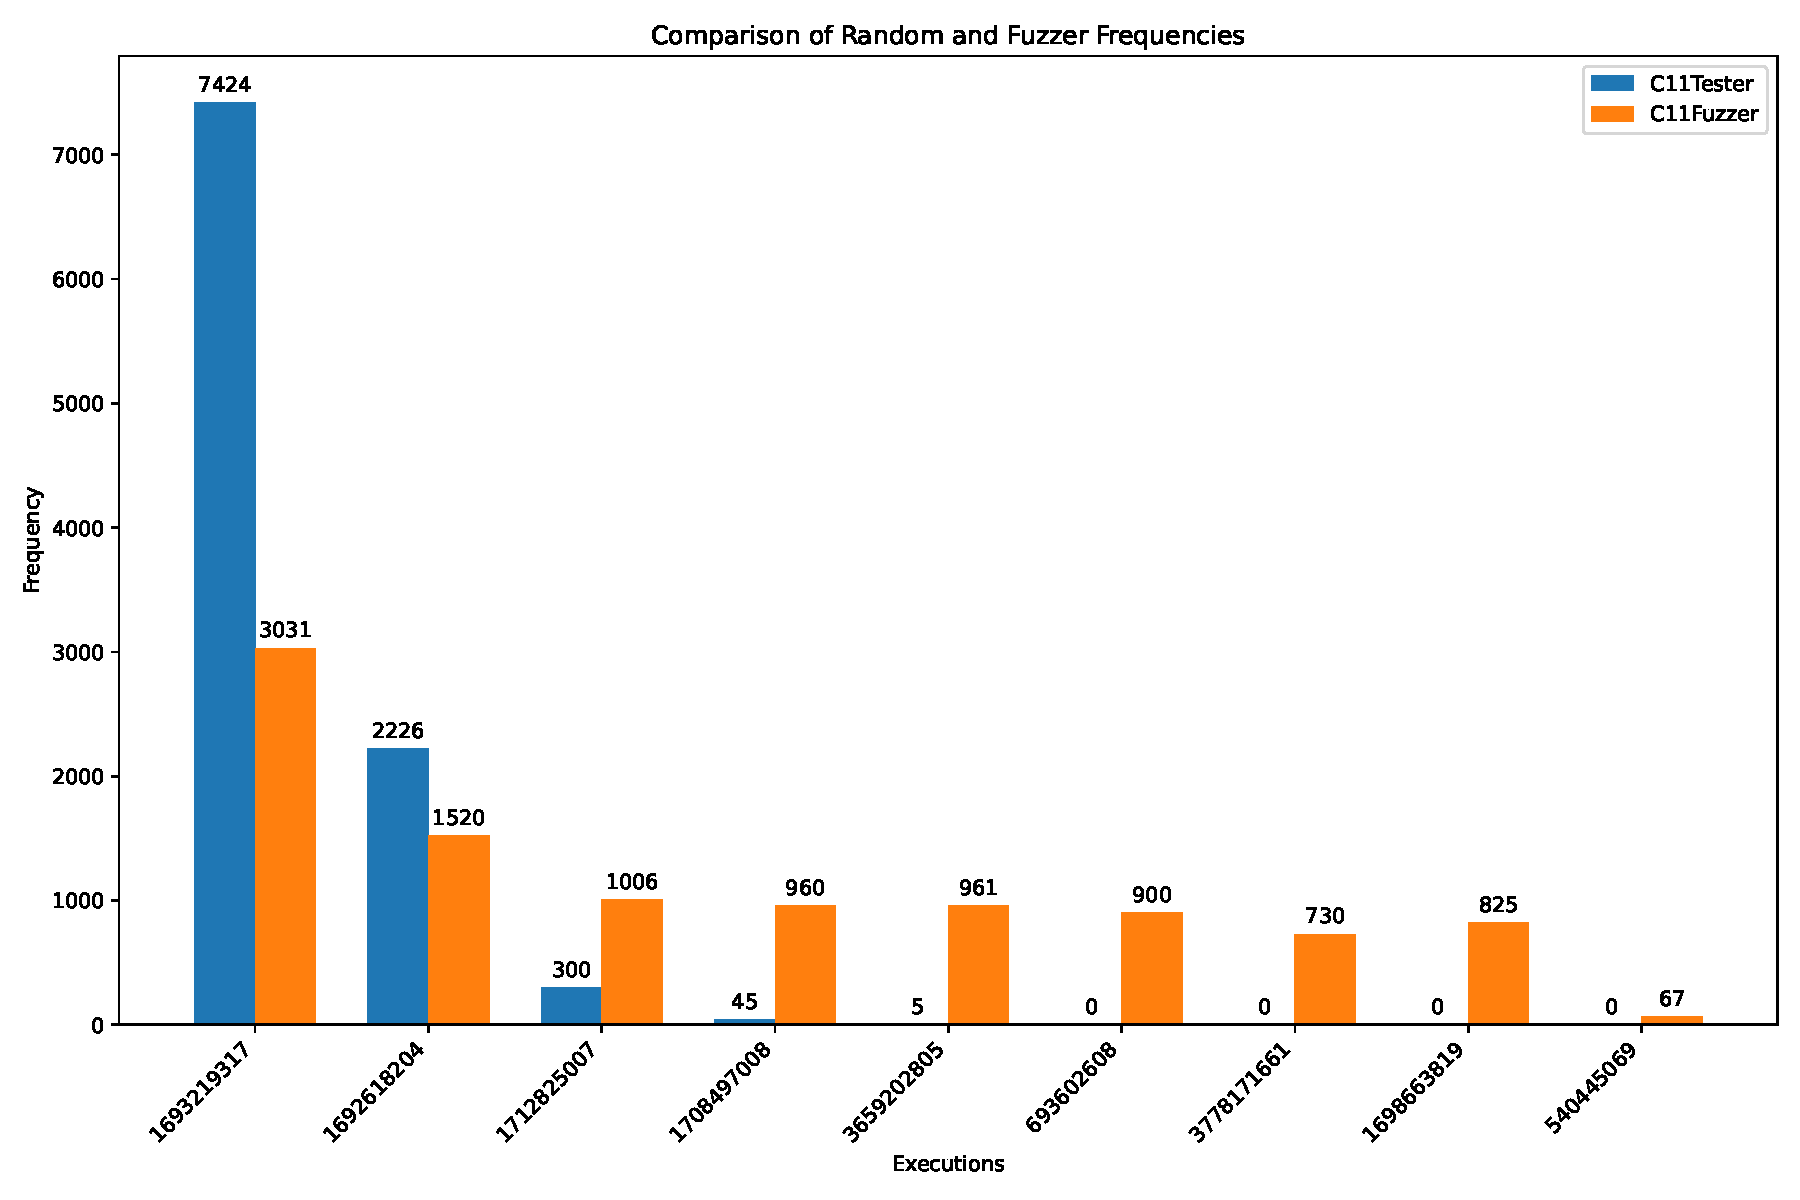
\includegraphics[scale=0.35]{figure/hardbug/long-race_freq.pdf}  
    \caption{Frequencies of execution graphs } 
    \label{graph-freq} 
\end{figure}
\michalis{Is there a better way to visualize this?}

\begin{figure}[H]

	\centering
	\begin{minipage}{0.45\textwidth}
		\centering
		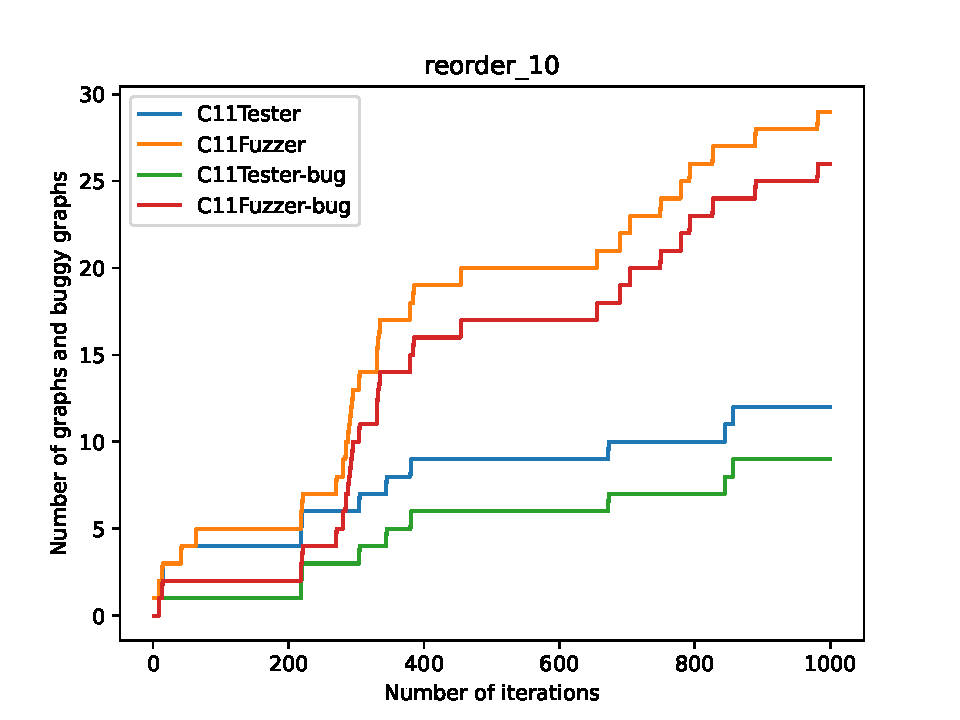
\includegraphics[width=\textwidth]{figure/hardbug/reorder_10_bug.pdf}
	\end{minipage}
	\hfill
	\begin{minipage}{0.45\textwidth}
		\centering
		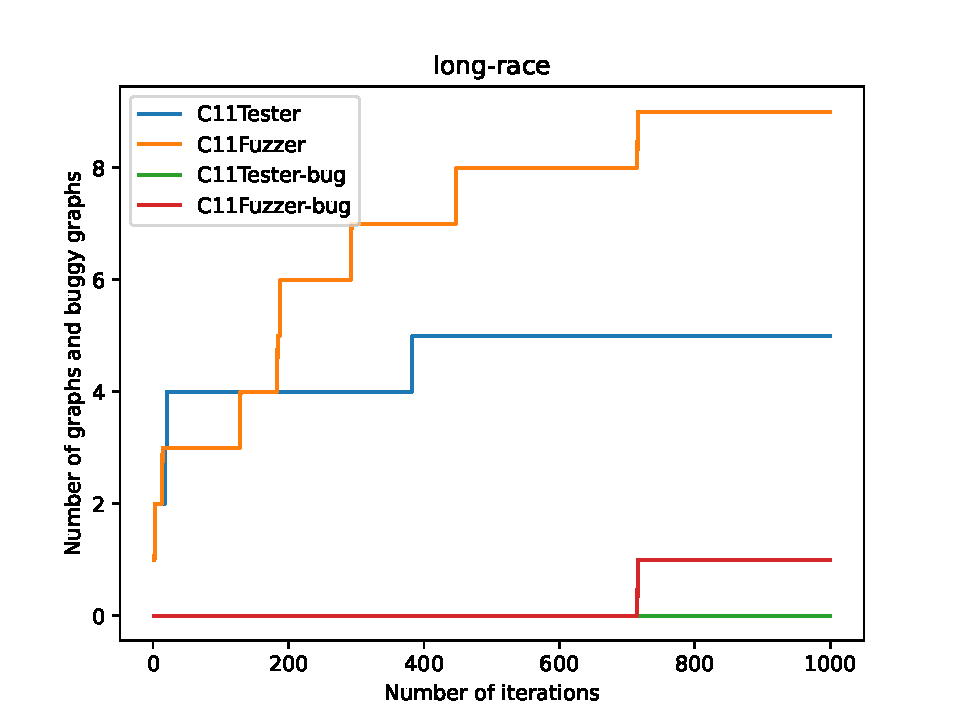
\includegraphics[width=\textwidth]{figure/hardbug/long-race_bug.pdf}
	\end{minipage}

	\vspace{0.5cm}

	\begin{minipage}{0.45\textwidth}
		\centering
		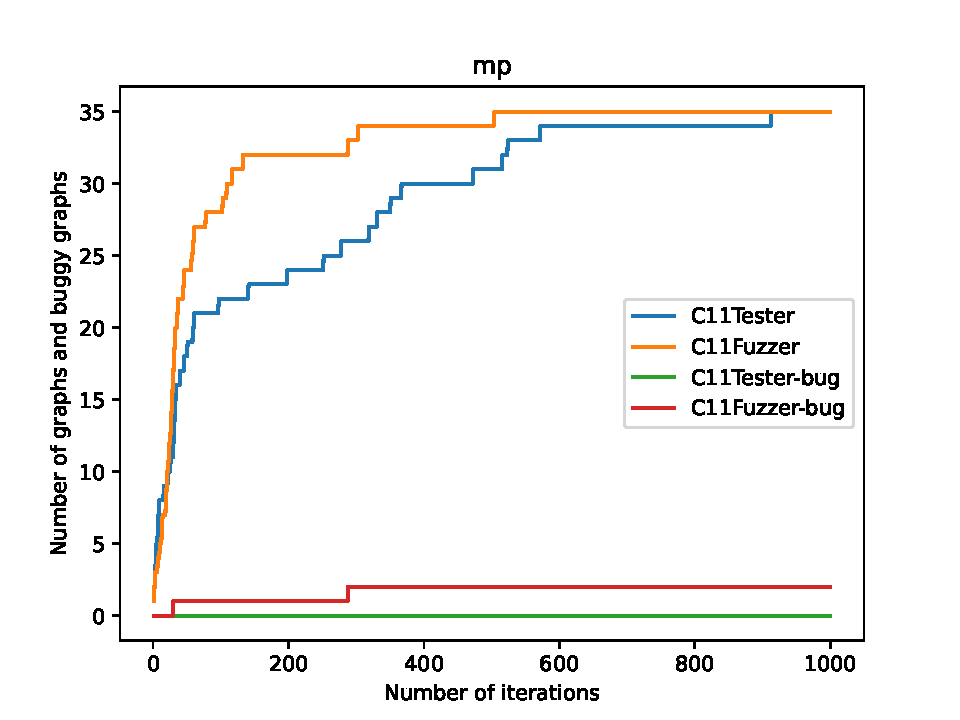
\includegraphics[width=\textwidth]{figure/hardbug/mp_bug.pdf}
	\end{minipage}
	\hfill
	\begin{minipage}{0.45\textwidth}
		\centering
		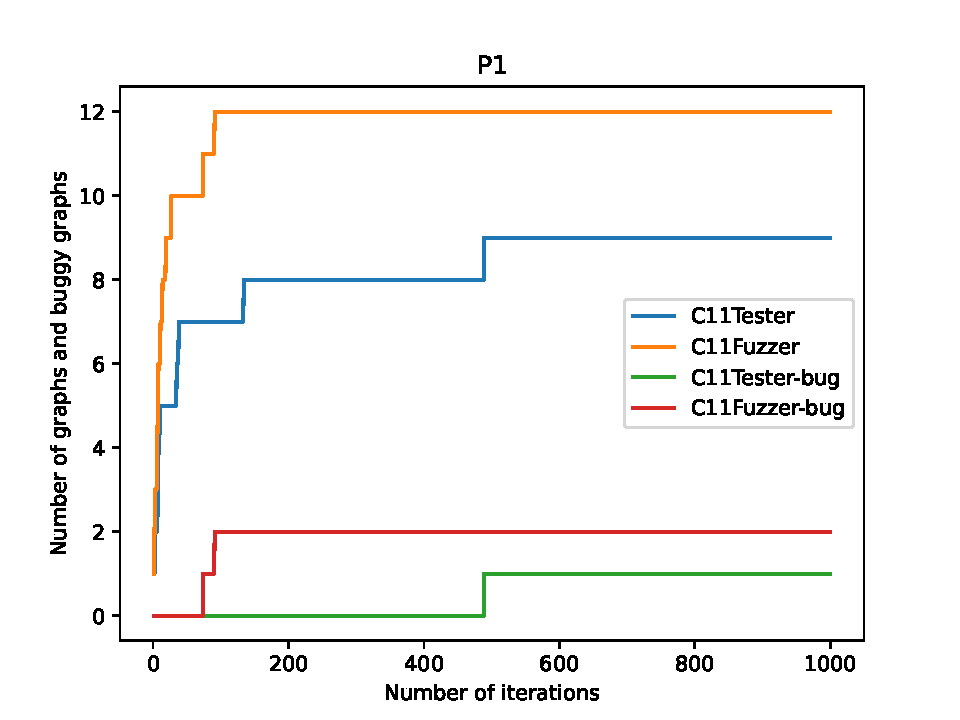
\includegraphics[width=\textwidth]{figure/hardbug/P1_bug.pdf}
	\end{minipage}
	\caption{Buf finding plots}
	\label{c11tester:bug-plot}

\end{figure}










\subsection{\ref*{RQ:coverage}: Fuzzer vs C11Tester}

Using the 11 benchmarks, we evaluate the ability of both the fuzzer and C11Tester to find unique execution graphs. The metric used is the number of different execution graphs discovered over $N$ iterations. Table~\ref{c11fuzzer-bench1} and Table~\ref{c11fuzzer-bench2} show the number of unique executions found by two approaches. It can be seen that the fuzzer is able to find a larger number of different execution graphs in a fixed number of iterations than C11Tester with the random-based searching strategy in most of the benchmarks, with the average improvement of 27.0\%. The improvements are calculated by:
\[
	R_{improvement} = \frac{N_{c11Fuzzer} - N_{c11Tester} }{N_{c11Tester} } \times 100 \% ,
\]
where $N_{c11Fuzzer}$ and $N_{c11Tester}$ are the number of unique execution graphs found by C11Tester and C11Fuzzer, respectively.

\begin{table}[h!]
	\begin{tabular}{ |c|ccccc| }
		\hline
		Benchmarks  & barrier & chase-lev-deque & mpmc-queue & linuxrwlocks & mcs-lock \\
		\hline
		C11Tester   & 6969    & 6244            & 4185       & 981          & 9703     \\
		C11Fuzzer   & 7741    & 8505            & 6373       & 1225         & 9994     \\
		\hline
		Improvement & 11.1\%  & 36.2\%          & 52.3\%     & 24.9\%       & 3.0\%    \\
		\hline
	\end{tabular}
	\caption{Benchmarks (1)}
	\label{c11fuzzer-bench1}

\end{table}

\begin{table}[h!]
	\begin{tabular}{ |c|cccccc| }
		\hline
		Benchmarks  & dekker & rwlock-test & seqlock-test & bipartite-buf & left-right & ring-buf \\
		\hline
		C11Tester   & 395    & 9998        & 6137         & 297           & 5378       & 328      \\
		C11Fuzzer   & 494    & 9997        & 7962         & 340           & 6678       & 576      \\
		\hline
		Improvement & 25.1\% & -0.0\%      & 29.7\%       & 14.5\%        & 24.2\%     & 75.6\%   \\
		\hline
	\end{tabular}
	\caption{Benchmarks (2)}
	\label{c11fuzzer-bench2}
\end{table}


Figure~\ref{c11tester:cov-plts2} and Figure~\ref{c11tester:cov-plts2} draw the coverage plots for each benchmark, with orange lines representing the fuzzer and blue lines representing the random tester. It can be observed that in all of these cases, the fuzzer is able to find more unique executions. In addition, in some benchmarks, such as chase-lev-deque or mpmc-queue, the fuzzer's speed of finding executions (the slop of coverage plost) does not significantly slow down as the number of found executions grows. Some coverage plots of the fuzzer, such as those in bipartite-buf and ring-buf, also have some "bumps" which the random tester do not have. Such bumps are caused by some prefixes that guide to a group of new interesting executions.

\begin{figure}[H]
    \centering

    \begin{minipage}{0.45\textwidth}
        \centering
        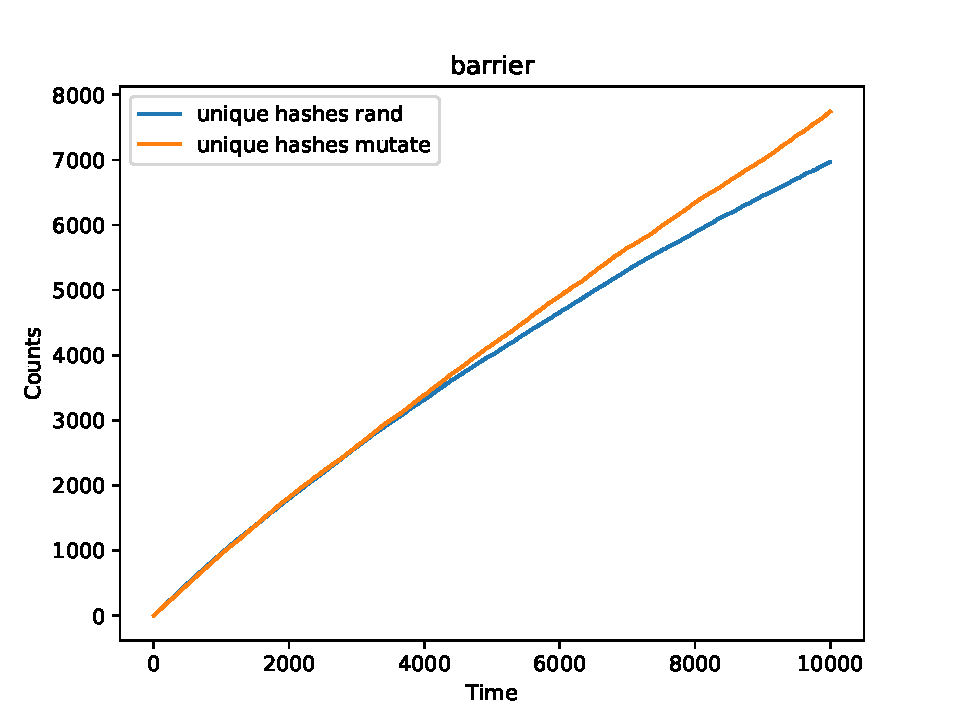
\includegraphics[width=\textwidth]{figure/barrier.pdf}
    \end{minipage}
    \hfill
    \begin{minipage}{0.45\textwidth}
        \centering
        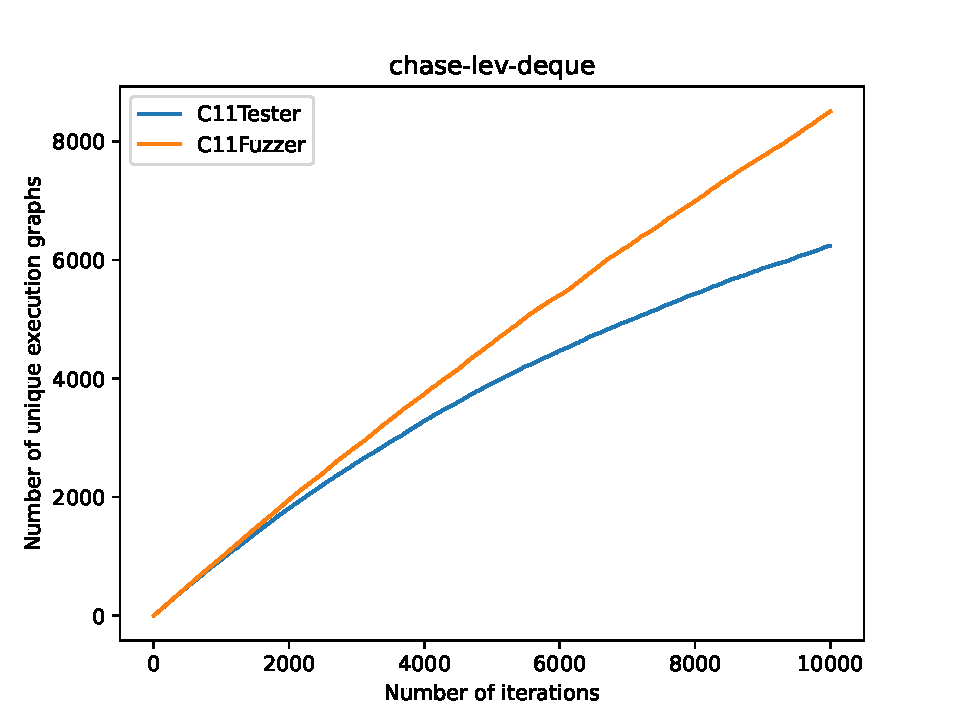
\includegraphics[width=\textwidth]{figure/chase-lev-deque.pdf}
    \end{minipage}

    \vspace{0.5cm}

    \begin{minipage}{0.45\textwidth}
        \centering
        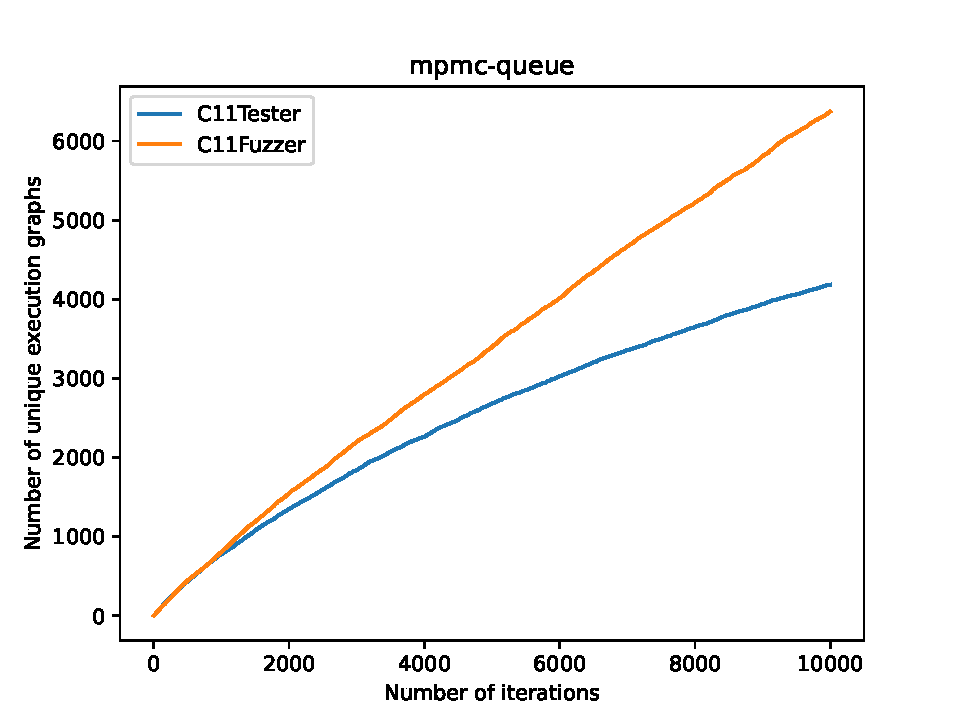
\includegraphics[width=\textwidth]{figure/mpmc-queue.pdf}
    \end{minipage}
    \hfill
    \begin{minipage}{0.45\textwidth}
        \centering
        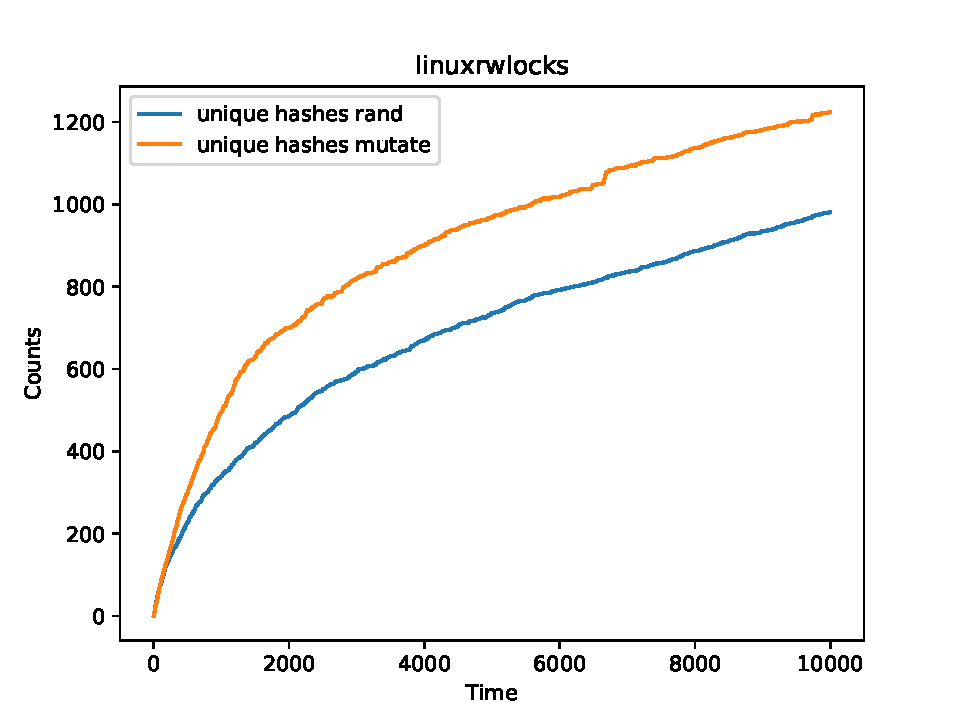
\includegraphics[width=\textwidth]{figure/linuxrwlocks.pdf}
    \end{minipage}

    \vspace{0.5cm}

    \begin{minipage}{0.45\textwidth}
        \centering
        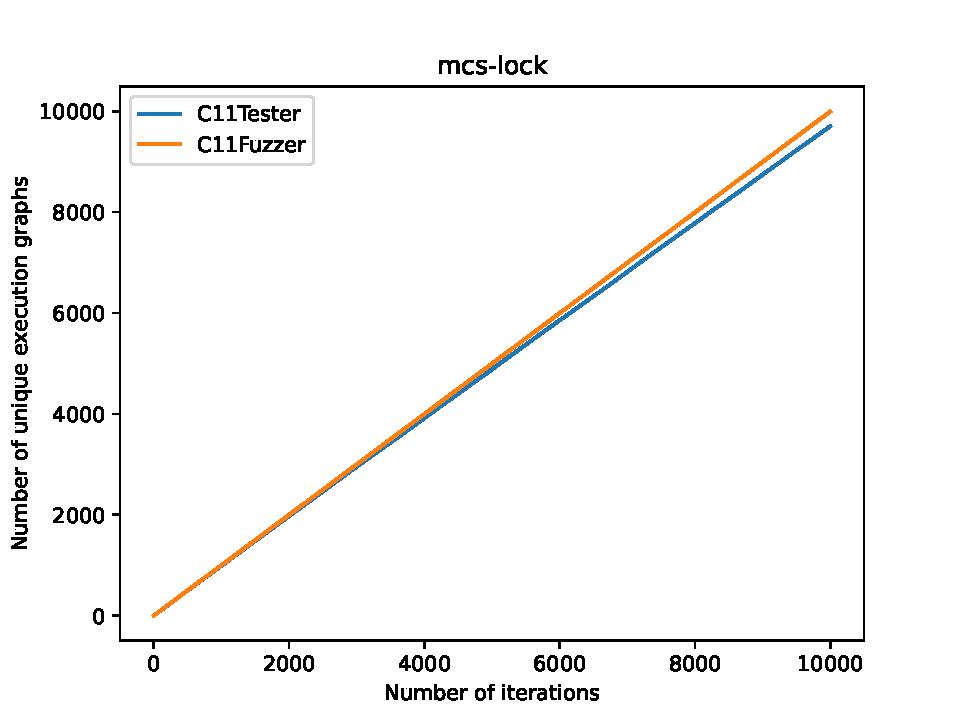
\includegraphics[width=\textwidth]{figure/mcs-lock.pdf}
    \end{minipage}
    \hfill
    \begin{minipage}{0.45\textwidth}
        \centering
        % This empty minipage will help the last image to be aligned to the left
    \end{minipage}

    \caption{Coverage plots (1)}
    \label{c11tester:cov-plts1}
\end{figure}


\begin{figure}[H]
    \centering
    \begin{minipage}{0.45\textwidth}
        \centering
        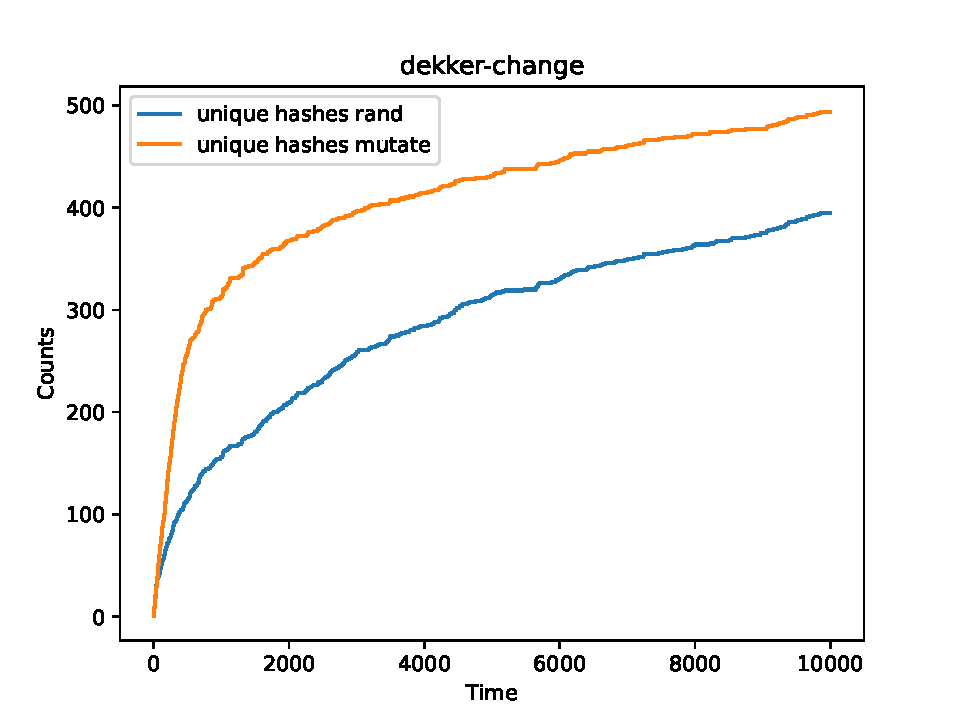
\includegraphics[width=\textwidth]{figure/dekker-change.pdf}
    \end{minipage}
    \hfill
    \begin{minipage}{0.45\textwidth}
        \centering
        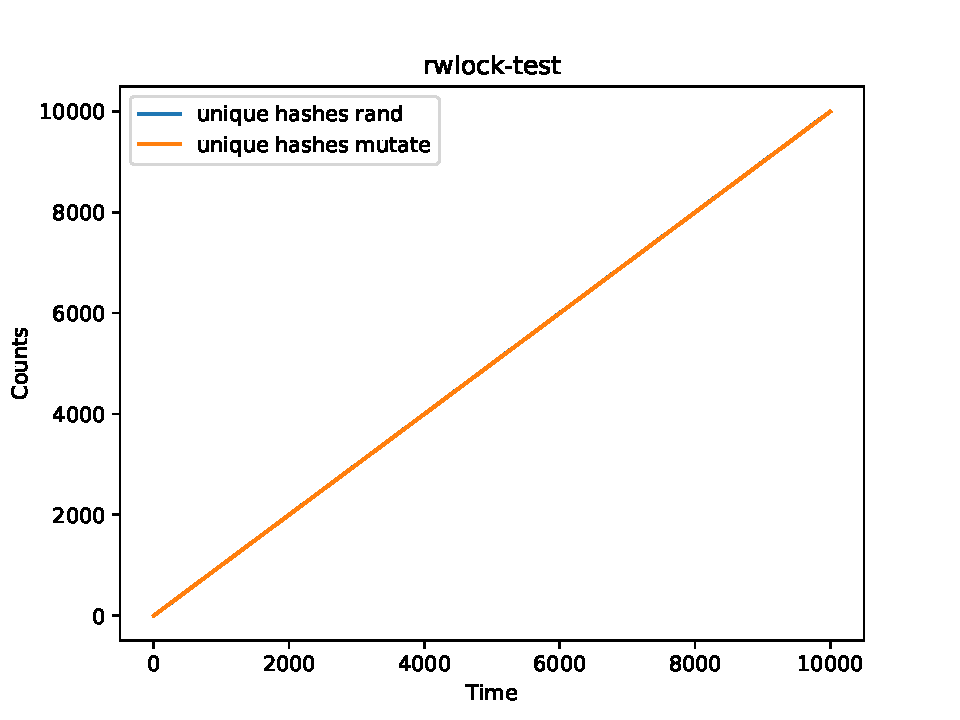
\includegraphics[width=\textwidth]{figure/rwlock-test.pdf}
    \end{minipage}

    \vspace{0.5cm}

    \begin{minipage}{0.45\textwidth}
        \centering
        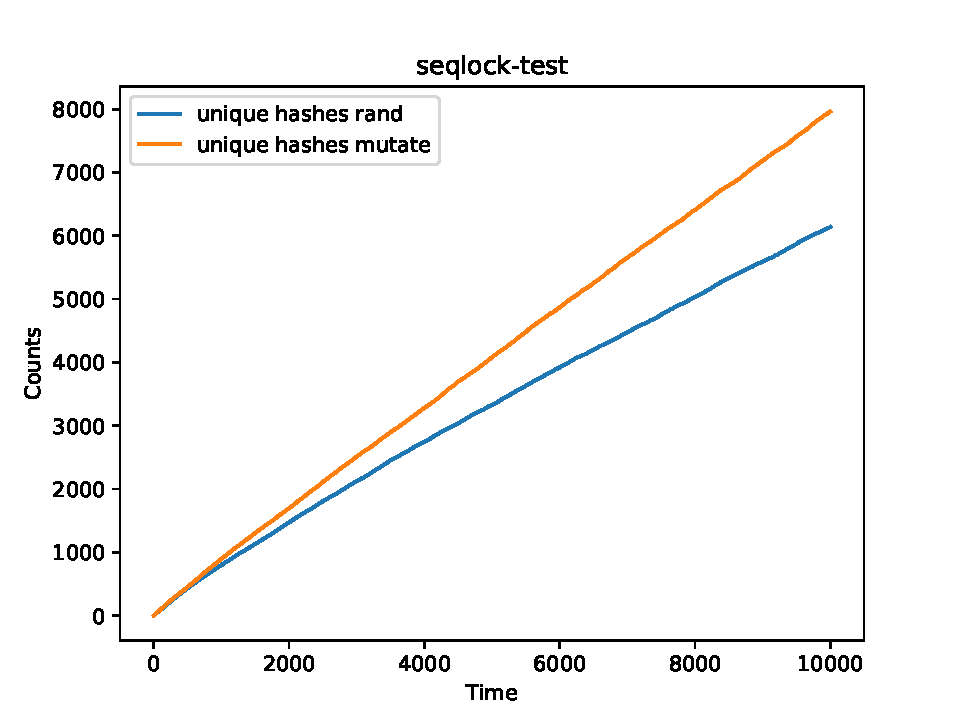
\includegraphics[width=\textwidth]{figure/seqlock-test.pdf}
    \end{minipage}
    \hfill
    \begin{minipage}{0.45\textwidth}
        \centering
        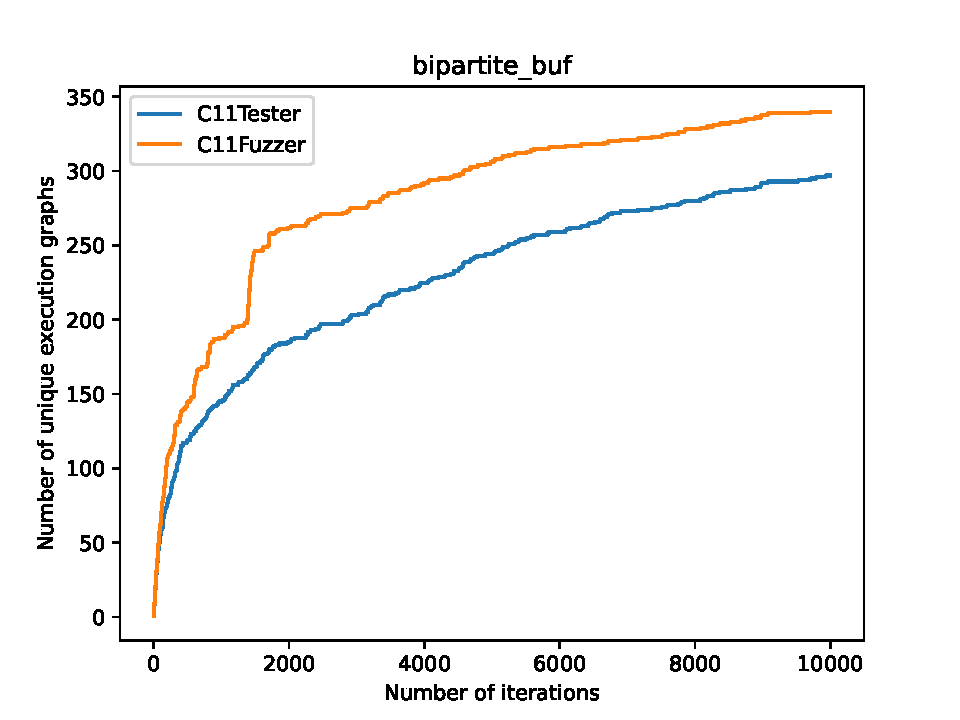
\includegraphics[width=\textwidth]{figure/bipartite_buf.pdf}
    \end{minipage}

    \vspace{0.5cm}

    \begin{minipage}{0.45\textwidth}
        \centering
        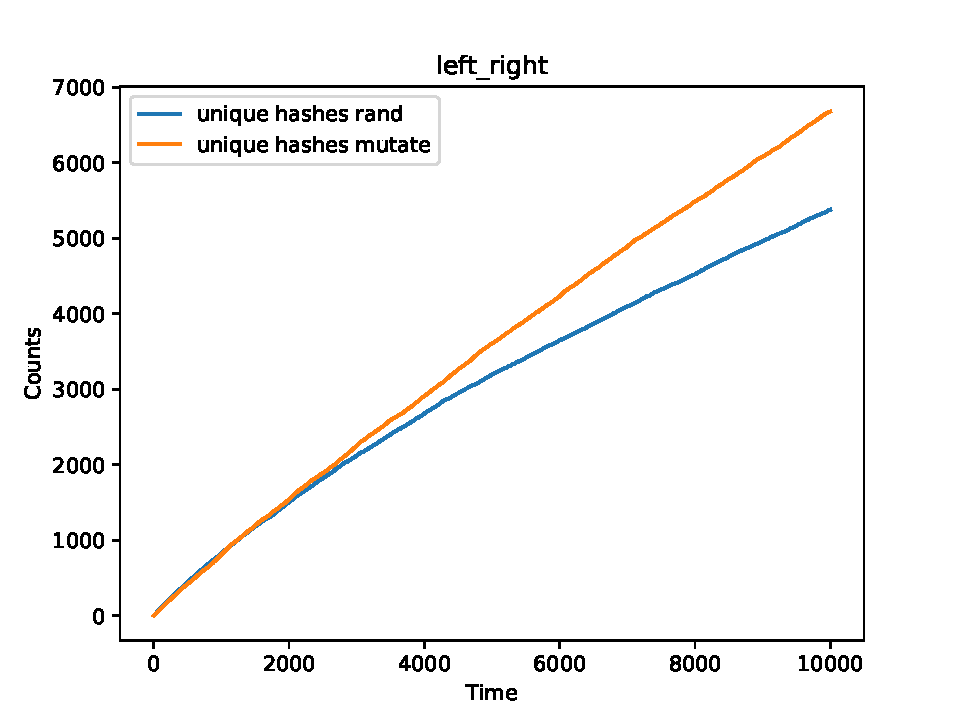
\includegraphics[width=\textwidth]{figure/left_right.pdf}
    \end{minipage}
    \hfill
    \begin{minipage}{0.45\textwidth}
        \centering
        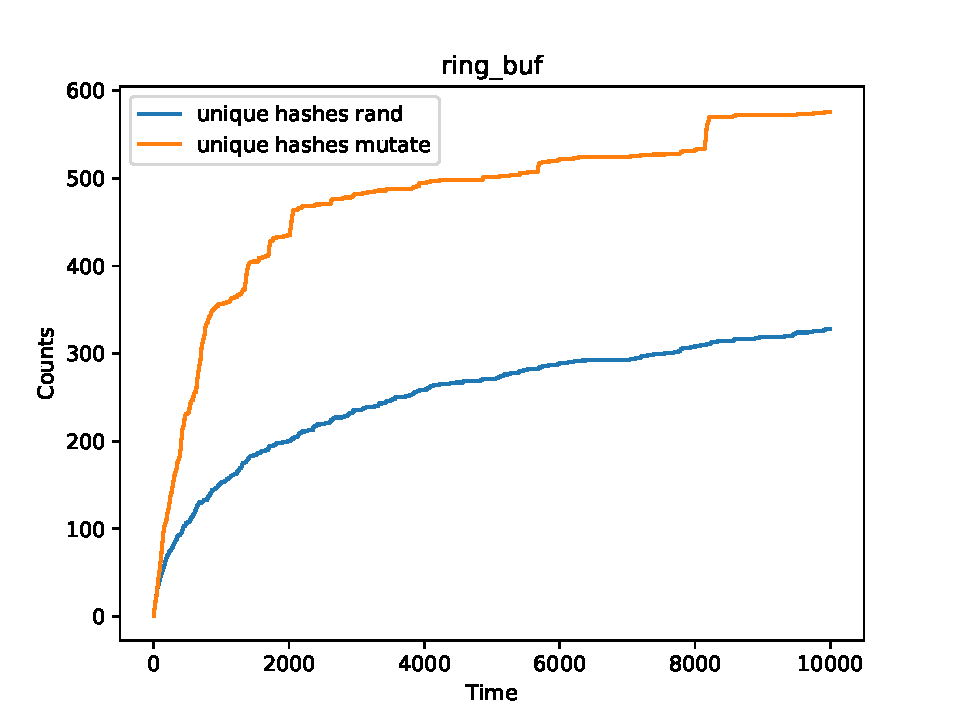
\includegraphics[width=\textwidth]{figure/ring_buf.pdf}
    \end{minipage}

    \caption{Coverage plots (2)}
    \label{c11tester:cov-plts2}
\end{figure}




\michalis{Why are there so many small figures and not a big one with many plots? (also below)}



\subsection{\ref*{RQ:coverage}: C11Fuzzer vs PCTWM}

PCTWM \cite{pctwm} is a state-of-the-art weak concurrency tester that expands the idea of PCT, which constrains the cope of exploring executions. It is expected that PCTWM will cover a smaller range of execution graphs than C11Tester, which performs an unbounded random search. A subset of the benchmarks described above is tested with the same configurations of bug depth and communication events, as shown in Table \ref{pctwm-configs}.

\begin{table}[h]
	\centering
	\begin{tabular}{ |c|ccc| }
		\hline
		Benchmark       & bug depth (d) & communication (k) & history (h) \\
		\hline
		barrier         & 1             & 10                & 2           \\
		chase-lev-deque & 2             & 56                & 1           \\
		mcs-lock        & 1             & 16                & 1           \\
		seqlock-test    & 4             & 18                & 1           \\
		linuxrwlocks    & 5             & 100               & 10          \\
		mpmc-queue      & 2             & 17                & 2           \\
		\hline
	\end{tabular}
	\caption{PCTWM parameters}
	\label{pctwm-configs}
\end{table}

Figure~\ref{fig:fuzz-vs-pctwm} shows the coverage plots of number of unique executions found by PCTWM, C11Fuzzer and C11Tester. It can be observed that PCTWM's bounded searching scope is usually smaller than C11Tester's unbounded random searching scope, which is smaller than C11Fuzzer's.


\begin{figure}[H]
    \centering

    \begin{minipage}{0.45\textwidth}
        \centering
        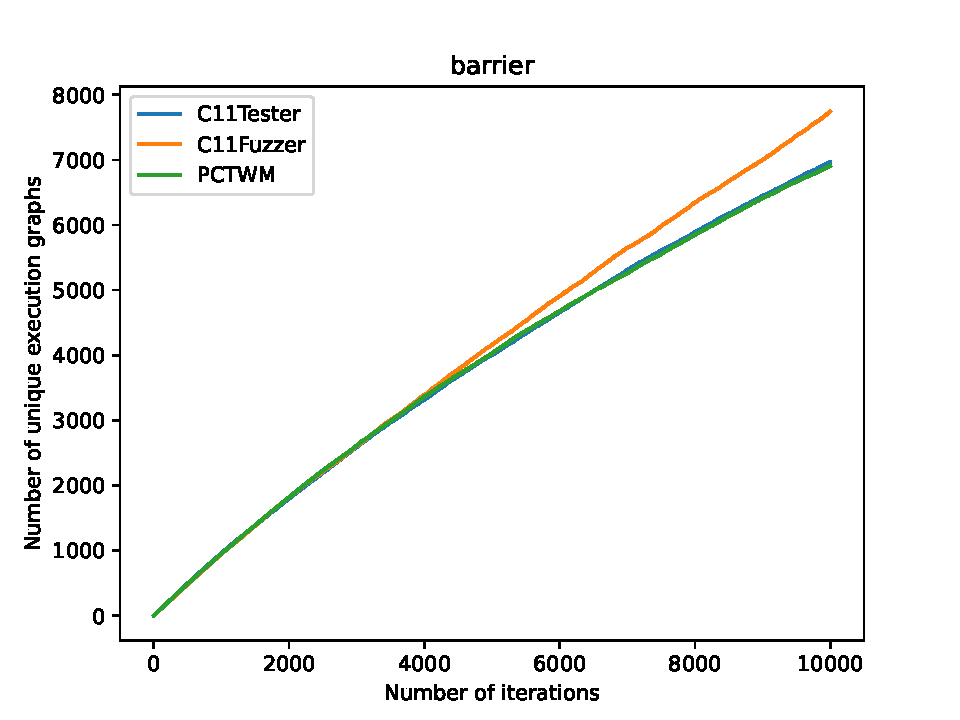
\includegraphics[width=\textwidth]{figure/pctwm/barrier.pdf}
    \end{minipage}
    \hfill
    \begin{minipage}{0.45\textwidth}
        \centering
        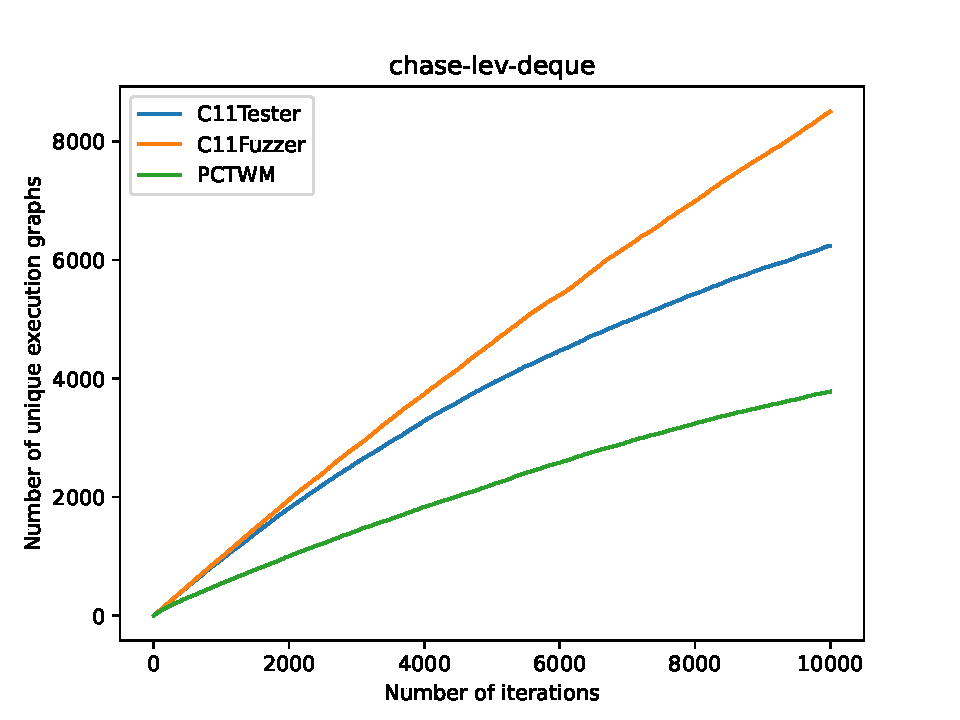
\includegraphics[width=\textwidth]{figure/pctwm/chase-lev-deque.pdf}
    \end{minipage}
    \vspace{0.5cm}

    \begin{minipage}{0.45\textwidth}
        \centering
        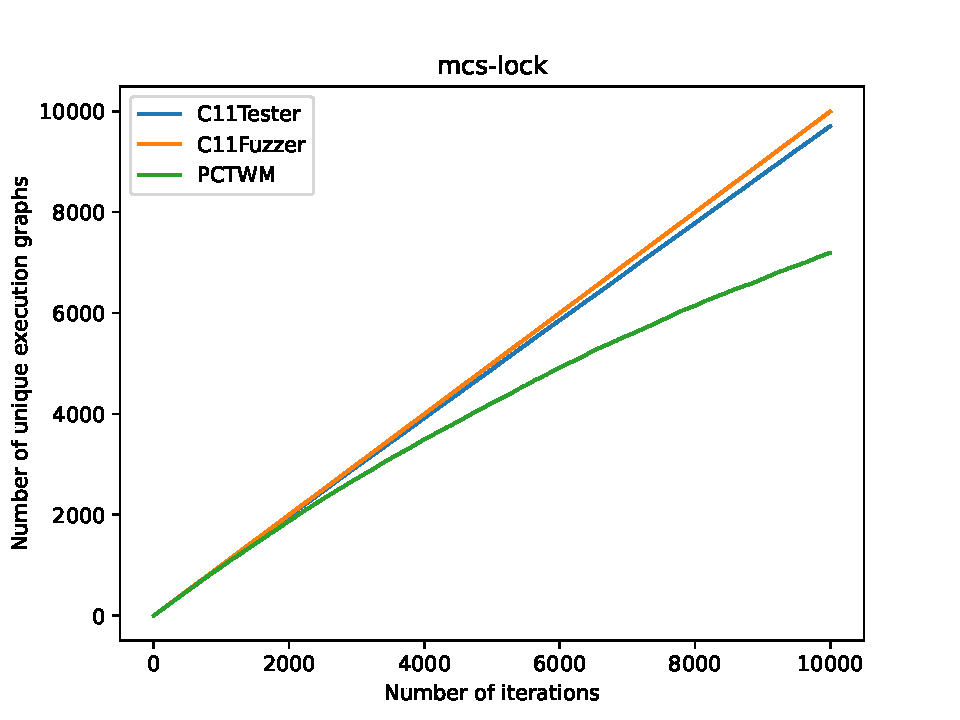
\includegraphics[width=\textwidth]{figure/pctwm/mcs-lock.pdf}
    \end{minipage}
    \hfill
    \begin{minipage}{0.45\textwidth}
        \centering
        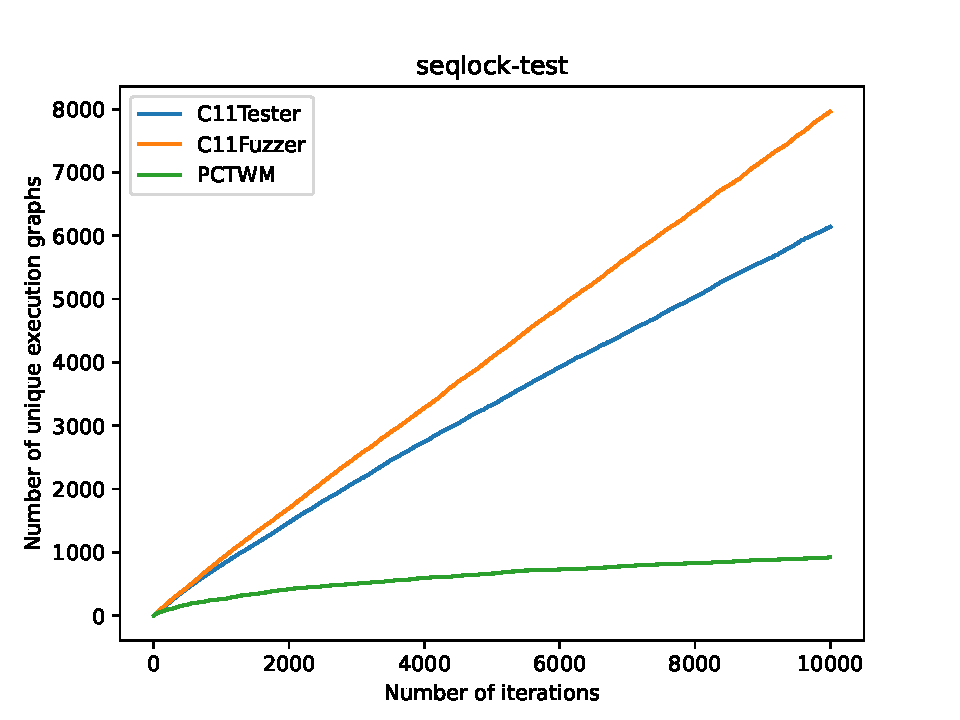
\includegraphics[width=\textwidth]{figure/pctwm/seqlock-test.pdf}
    \end{minipage}
    \vspace{0.5cm}

    \begin{minipage}{0.45\textwidth}
        \centering
        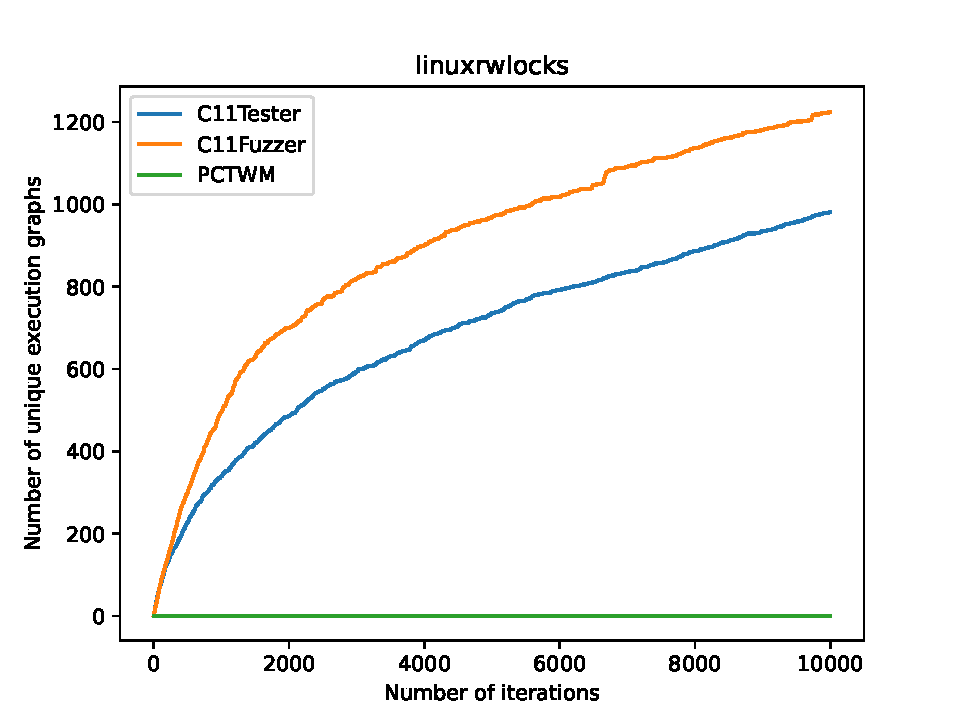
\includegraphics[width=\textwidth]{figure/pctwm/linuxrwlocks.pdf}
    \end{minipage}
    \hfill
    \begin{minipage}{0.45\textwidth}
        \centering
        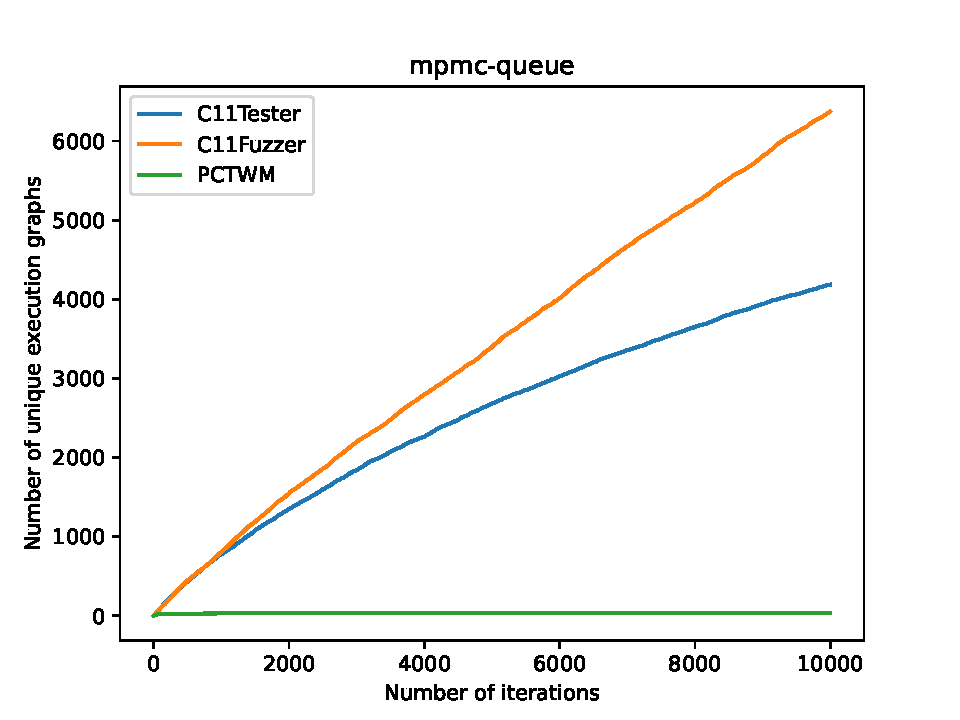
\includegraphics[width=\textwidth]{figure/pctwm/mpmc-queue.pdf}
    \end{minipage}
    \vspace{0.5cm}

    \caption{C11Fuzzer vs PCTWM}
    \label{fig:fuzz-vs-pctwm}
\end{figure}



\subsection{\ref*{RQ:bug}: Bug hitting rate}

The design of the fuzzer is not biased towards finding bugs, but it is also interested whether covering a wider range of execution graphs will improve the bug hitting rate. Some of the above benchmarks contain injected bugs, such as the inappropriate use of synchronization primitives, which can introduce either data races or assertion failures. The bug hitting rate is computed as:
\[
	R_{bug} = \frac{N_{bug}}{N},
\]
where $N_{bug}$ is the number of different buggy executions found over $N$ iterations. Since all benchmarks are executed $N$ times, higher number of bugs represent higher bug hitting rate. Table \ref{buggy1} and \ref{buggy2} show the results from the benchmarks.


\begin{table}[h!]
	\begin{tabular}{ |c|ccccc| }
		\hline
		Benchmarks & barrier & chase-lev-deque & mpmc-queue & linuxrwlocks & mcs-lock \\
		\hline
		C11Tester  & 5789    & 5895            & 2341       & 976          & 8525     \\
		C11Fuzzer  & 6993    & 5858            & 5858       & 1220         & 9418     \\
		\hline
	\end{tabular}
	\caption{Bug hitting rate (1)}
	\label{buggy1}

\end{table}

\begin{table}[h!]
	\begin{tabular}{ |c|cccccc| }
		\hline
		Benchmarks & dekker & rwlock-test & seqlock-test & bipartite-buf & left-right & ring-buf \\
		\hline
		C11Tester  & 5      & 4697        & 3872         & 297           & 1478       & 328      \\
		C11Fuzzer  & 5      & 4736        & 5009         & 340           & 1488       & 576      \\
		\hline
	\end{tabular}
	\caption{Bug hitting rate (2)}
	\label{buggy2}
\end{table}

It can be observed that except for dekker benchmark, which in total has 5 different bugs, C11Fuzzer is able to find more bugs in other benchmarks.


\subsection{\ref*{RQ:overhead}: Real-world applications}

The fuzzer is composed of a python script that performs mutation and file IO's and a compiled binary that is hooked to the executed program. For overhead evaluation, several things are measured:
\begin{itemize}
	\item The scripting overhead of the random version and the fuzzing version. Substracting them yields the overhead of mutation and IO's.
	\item The time used by the binary to load the decisions for replay.
	\item The time used for the binary to execute.
\end{itemize}

We test our fuzzer using a real-world application, iris, which is an asynchronous logging library that makes extensive use of atomic operations. Both C11Tester and C11Fuzzer are tested $N=100$ times and an average of the overhead per execution is taken. Table \ref{overhead} shows the measurement results. It can be seen that the mutation takes up most of the overhead. A future improvement could be writing the fuzzer in a compiled language and transfer the heavy file IO into memory.

\begin{table}[h!]
	\centering
	\begin{tabular}{ |c|cccc| }
		\hline
		Items     & script & binary & mutation & load-replay \\
		\hline
		C11Tester & 1.50s  & 39.51s & 0s       & 0s          \\
		C11Fuzzer & 8.9s   & 40.5s  & 7.4s     & 2.9s        \\
		\hline
	\end{tabular}
	\caption{Overhead (per execution)}
	\label{overhead}
\end{table}

% \burcu{TODO: Discuss the results/plots. What do we observe? What can we say about the results?}

\michalis{Why not profile C11Fuzzer and see the percentage of mutation?}
\michalis{Also, I'm not sure how to read this table. Is it that there are 7.4secs of overhead at each execution, for 1000 executions? Why not just take 1000 iterations K times and average them w/ C11Tester and C11Fuzzer, respectively? }